\documentclass[10pt]{beamer}
\usetheme{Warsaw}
\usepackage[utf8]{inputenc}
\usepackage[spanish]{babel}
\usepackage{amsmath}
\usepackage{amsfonts}
\usepackage{amssymb}
\usepackage{graphicx}
\author{Luis Clemente Michicol Martinez\\
Jorge Ramos Herrera}
\title{Aplicación del método Markov Chain Monte Carlo en cosmología}
%\setbeamercovered{transparent} 
%\setbeamertemplate{navigation symbols}{} 
%\logo{} 
\institute{Benemérita Universidad Autónoma de Puebla} 

%\subject{} 
\begin{document}

\begin{frame}
\titlepage
\end{frame}

%\begin{frame}
%\tableofcontents
%\end{frame}

\begin{frame}{Introducción}
El objetivo es aplicar el método numérico MCMC (Markov Chain Monte Carlo), en concreto se aplica para determinar los parámetros del modelo cosmologico basado en la métrica de Friedmann-Lemaître-Robertson-Walker, por medio de las observaciones cosmologicas de luz emitida por \textbf{candelas estándar}.
\end{frame}

\begin{frame}{¿De donde sale MCMC?}

El método MCMC forma parte de un conjunto de métodos numéricos conocidos como métodos estadísticos Bayesianos, pero ¿Por qué métodos estadísticos Bayesianos?. Se les conoce de esta manera ya que se derivan del \textbf{teorema de Bayes}.

\begin{equation}
	P(A\mid B) = P(A) \frac{P(B\mid A)}{P(B)}
\end{equation}

Este tipo de métodos se usan para determinar distribuciones probabilidad posteriores, y en realidad existen distintos tipos de métodos a parte de MCMC, sin embargo, en este caso se limita únicamente a MCMC.

\end{frame}

\begin{frame}
Ahora contextualizando, el método MCMC se puede entender en dos partes, como primera parte Monte Carlo, es un método que mediante generación de números aleatorios se busca hacer una aproximación de una cantidad, un ejemplo muy común es el de aproximar el valor de $\pi$ como se muestra en la figura.
\begin{center}
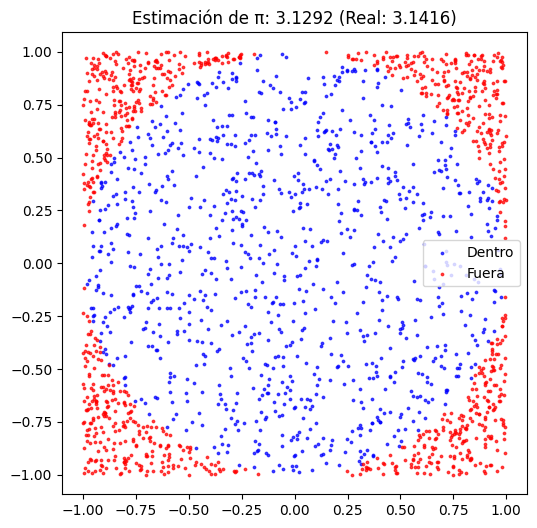
\includegraphics[scale=0.4]{SimM.png} 
\end{center}


\end{frame}

\begin{frame}
Por otra parte una cadena de Markov (o Markov Chain), es una secuencia de eventos, de los cuales únicamente forman una cadena de Markov aquellos que cumplan que la probabilidad del evento $X_{n+1}$ solo dependa del evento $X_n$, es decir que el evento subsecuente dependa del evento presente, esto también se les conoce como cadenas de Markov con memoria a corto plazo.
Algo importante de las cadenas de Markov, es que tienden a un estado estacionario, este estado, para este caso es nuestra distribución posterior $P(A\mid B)$.
Entonce la combinación de ambos métodos da MCMC.
\end{frame}

\begin{frame}{Algoritmo de Metropolis-Hastings}
Además del método MCMC, se requiere el algoritmo de Metropolis-Hastings, el cual nos va asegurar la convergencia a la distribución posterior, el algoritmo es el siguiente.

\begin{itemize}
\item Se inicializa $x_0$ como un estado inicial, esto puede ser de manera arbitraria, o bajo ciertas condiciones.
\item Se propone un posible candidato $x$, el cual tendrá una cierta distribución, la cual se recomienda que sea simétrica para que se simplifiquen los cálculos. Ahora se calcula la probabilidad de aceptación la cual esta dada por lo siguiente.
\begin{equation}
\alpha = min\left(1,\frac{P(D\mid x)q(x_0\mid x)}{P(D\mid x_0)q(x\mid x_0)}\right)
\end{equation}
En caso de que la distribución de $x$ es simétrica, es decir, $q(x_0\mid x)=q(x\mid x_0)$
Entonce se reduce a 
\begin{equation}
\alpha = min\left(1,\frac{P(D\mid x)}{P(D\mid x_0)}\right)
\end{equation}
\end{itemize}

\end{frame}

\begin{frame}
\begin{itemize}
\item Finalmente, para decidir si se acepta o no el candidato, es generando un número aleatorio $u$ con distribución uniforme $[0,1]$.

\begin{itemize}
\item Si $u\leq \alpha$ se acepta el candidato $x_{t+1} = x$
\item Si $u>\alpha$ se rechaza el candidato $x_{t+1}=x_t$
\end{itemize}

\end{itemize}

Ahora este algoritmo garantiza que se cumpla el balance detallado, lo que garantiza la convergencia a la distribución posterior.
\end{frame}

\begin{frame}{Aplicación en cosmologia.}
Para abordar esto, se tiene que encontrar la relacion que hay entre la distancia luminosa, y el modelo cosmologico, esto debido a que como se menciono en la introducción los datos que se utilizaron para aplicar el método MCMC, son mediciones de intensidad de luz, emitida por las candelas estándar.
La velocida de recesión esta dada por la siguiente expresión.

\begin{equation}
v_r = H_0 d_L
\end{equation}

Por otra parte las coordenada comoviles se expresna de la forma.

\begin{equation}
r = a(t)x
\end{equation}
donde $a(t)$ se conoce como el factor de escala, si se le saca la derivada temporal.

\begin{equation}
v_r = \dot{r} = \frac{\dot{a}}{a}ax + a\dot{x}
\end{equation}
\end{frame}

\begin{frame}
Ahora se pude definir la tasa de Hubble como 
\begin{equation}
H(t) = \frac{\dot{a}}{a}
\end{equation}

De esta manera la expresión (6) queda de la siguiente manera.

\begin{equation}
v_r = Hr
\end{equation}
\end{frame}

\begin{frame}{Corrimiento al rojo.}
Consideramos la relación $\lambda_{obs} = \lambda_{em} + \Delta\lambda$, donde $z = \Delta\lambda / \lambda_{em}$, entonces obtenemos.

\begin{equation}
\frac{\lambda_{obs}}{\lambda_{em}} = 1 + z
\end{equation}

Existe una relación entre distancia comovil y distancia física, con la longitud de onda, el cual vine dada por $\lambda = a x$, es decir que la longitud de onda cumple la función de distancia comovil, de esta forma se puede relacionar lo siguiente.

\begin{equation}
\frac{\lambda_{obs}}{\lambda_{em}} = \frac{a(t_0)}{a(t_{em})} = \frac{1}{a}
\end{equation}

ya que generalmente $a(t_0) = 1$ se normaliza.Con lo cual ya nos queda la siguiente relación.

\begin{equation}
\frac{1}{a} = 1 + z
\end{equation}
\end{frame}

\begin{frame}{Metrica de LFRW}

La métrica LFRW esta dada por la siguiente expresión.

\begin{equation}
ds^2 = -c^2dt^2 + a(t)^2\left(\frac{dr^2}{1-Kr^2} + r^2(d\theta^2 + \sin^2\theta d\phi^2\right)
\end{equation}

Ahora se consideran coordenadas comoviles, y ademas viaja una señal sobre una geodésica que va de $r_0=0$ hasta $r$, donde $d\theta=d\phi=0$ ya que $\theta=cte$.

\begin{equation}
d\chi = \frac{dr}{\sqrt{1-Kr^2}}
\end{equation}

con lo cual la distancia que recorra es 
\begin{equation}
\chi = \int_0^r\frac{dr}{\sqrt{1-Kr^2}}
\end{equation}

\end{frame}

\begin{frame}{Ecuación de Friedmann}

Se parte de la ecuación de Einstein, que describe la dinámica y la geometría del universo.

\begin{equation}
R_{\mu\nu} - \frac{1}{2}g_{\mu\nu}R = 8\pi T_{\mu\nu}
\end{equation}

Haciendo algunas consideraciones y manipulando la expresión se llega a la ecuación de Friedmann

\begin{equation}
H^2 + \frac{k}{a^2} = \frac{8}{3}\pi\rho
\end{equation}

y esta misma se puede reescribir de la siguiente manera

\begin{equation}
\frac{k}{H^2a^2} = \frac{8\pi}{3H^2}\rho - 1
\end{equation}

Haciendo la consideración de que  $\rho_c = \frac{3H^2}{8\pi}$ que corresponde a la densidad critica, con lo cual se puede reescribir de la siguiente manera

\begin{equation}
\frac{k}{a^2H^2} = \Omega - 1
\end{equation}

\end{frame}

\begin{frame}{Ecuación de continuidad.}

Ahora al considerar la ecuación de continuidad.

\begin{equation}
\nabla_\mu T^{\mu\nu} = 0
\end{equation}

donde $T^{\mu\nu}$ es el tensor de energía momento, ademas $P = \omega\rho$

Al hacer esa consideración se obtiene lo siguiente.

\begin{equation}
\frac{\dot{\rho}}{\rho} = -3(1+\omega)\frac{\dot{a}}{a}
\end{equation}

se puede ver que al hacer las integrales de la anterior ecuación se obtiene lo siguiente.

\begin{equation}
\rho \varpropto a^{-3(1+\omega)}
\end{equation}

\end{frame}

\begin{frame}
Considerando los distintos contenidos del universo es decir.

\begin{itemize}
\item \textbf{Materia} $\dot{\rho}_m + 3H\rho_m = 0\rightarrow \rho_m\sim a^{-3}$
\item \textbf{Radiación} $\dot{\rho_r} + 4H\rho_r = 0 \rightarrow \rho_r\sim a^{-4}$
\item \textbf{Energía oscura} $\dot{\rho_\Lambda} = 0\rightarrow \rho_\Lambda = cte$
\end{itemize}

De esta manera se puede hacer la siguiente consideración.

\begin{equation}
\rho = \rho_m+\rho_r+\rho_\Lambda
\end{equation}

De la ecuación (16) se considera $k=0$ que corresponde con un universo plano, la ecuación de Friedmann y además  se toma en cuenta que $\Omega_i = \rho_i/\rho_c$ con esta consideraciones se obtiene lo siguiente.

\begin{equation}
\frac{H^2}{H_0^2} = \Omega_{r,0}a^{-4}+\Omega_{m,0}a^{-3} + \Omega_{\Lambda,0}
\end{equation}
\end{frame}

\begin{frame}{Distancia luminosa}
La distancia luminosa esta dada por 

\begin{equation}
d_L(z) = a_0(1+z)S_k(\chi(z))
\end{equation}

Y se define $\mu$  es una medida logarítmica de la distancia fuente.

\begin{equation}
\mu = 5\log_{10}\left(\frac{d_L}{10pc}\right)
\end{equation}

De esta manera podemos relacionar las observaciones de los objetos cosmologicos para utilizar el método MCMC.

\end{frame}
\end{document}